\section{Introduction}
\label{sec:Introduction}
Conventionally, the design of data structures and algorithms is chiefly focused on performance,
which is of significantly diminished concern in proof assistants. As such, proof assistants often
use entirely different data structures than those of conventional settings, with a focus on simplicity
or useful proof-theoretic properties. Dictionaries - which serve a broad range of purposes but are
perhaps most familiar in some implementations of type contexts and evaluation environments - are typically
implemented in one of the following manners: (TODO source for each)
\\\\
\newcommand{\lameq}[1]{$\lambda$ $x$ . $x == {#1}$}

\begin{figure*}
\begin{tabular}{ l l }
 Simple Association List (SAL)        & [(3, "c"), (1, "b"), {\color{gray} (3, "q")}, (6, "d")] \\
 Canonicalized Association List (CAL) & [(1, "b"), (3, "c"), (6, "d")] \quad (insert function dedupes and preserves canonical order) \\
 Finite Partial Function (FPF)        & \lameq{3} ? "c" : (\lameq{1} ? "b" : (\lameq{3} ? {\color{gray} "q"} : (\lameq{6} ? "d" : None) x) x) x
\end{tabular}
\caption{blah}
\end{figure*}

%% \\

The \sal~ (\SAL) solution is perhaps the most common, being trivially simple. Furthermore:
%\begin{itemize}
 (1) any \SAL~ that type-checks represents a valid mapping,
       so there's no need to refine the dict with a proof term that asserts its validity,
 (2) it's trivial to destruct and iterate,
 (3) checking semantic equivalence of two dicts, while non-trivial, is decidable and not too difficult.
%\end{itemize}
 The major downside is that many distinct dicts
represent the same semantic mapping - because dicts are sensitive to duplication and ordering
of insertions, semantically equivalent dicts may not be reflexively equal:
  %% \begin{figure}[H]
  \begin{figure*}
    \centering
    \begin{tikzpicture}[nodes = {align = left}]
      \node [scale=.45]
      {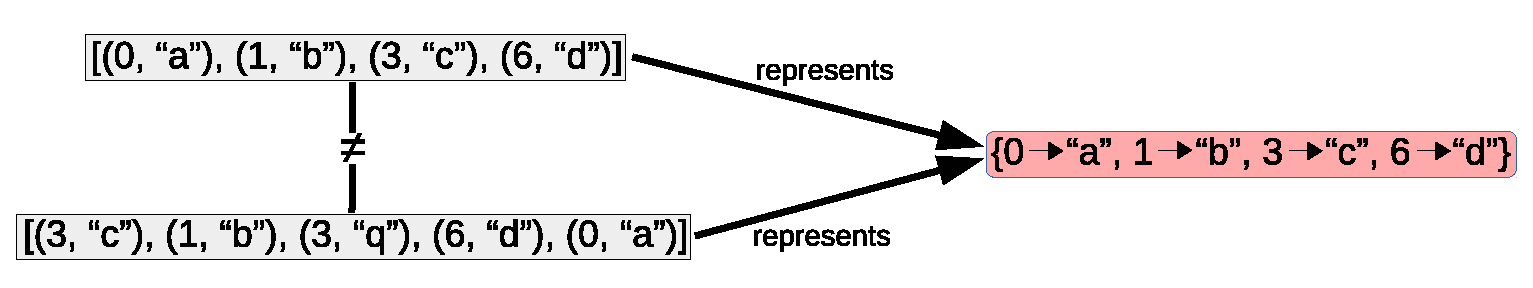
\includegraphics{figs/unequal.eps}};
    \end{tikzpicture}
    \caption{Same semantic mapping represented by unequal {\SAL}s}
    \label{fig:uneq}
  \end{figure*}
  %% \end{figure}
Developing proofs is challenging, so any stumbling block, such as the inability to use a built-in equality
primitive to establish semantic equivalence of two objects, or the awkwardness of packaging
proof terms with data (noting the difficulties that arise from proof relevance), can cause exorbitant
increases in verbosity, time, effort, and accidental complexity. Since performance is often not a concern,
we have an opportunity to reassess the core criteria by which data structures are judged. Chiefly, these
new criteria will focus on alleviating or eliminating difficulties that crop up in the development of
proofs. In the \nameref{sec:Problem} section, we discuss several of these properties and argue for their
conceptual and practical importance.

The \cal~ (\CAL) and \fpf~ (\FPF) solutions (as well as ours) are set-like - i.e. they are insensitive
to duplication and ordering of insertions. As such, semantically equivalent dicts are also equal according
to the built-in equality primitive\footnote{Finite partial functions require the additional postulate of
\emph{functional extensionality}, which can be postulated
at essentially no cost given that it's been proven consistent with the constructive calculi underlying most
popular proof assistants (TODO SOURCE)}. However, \CAL~ and \FPF~ have other drawbacks.
If used as data, a \CAL~ must be refined with a proof of validity to ensure that it is ordered and deduped,
while equality is not decidable for {\FPF}s. In the \nameref{sec:Problem} section we discuss the difficulties
that arise from these drawbacks.

Our solution, which we dub {\dd}s, addresses the aforementioned problems by using a delta to
encode a key relative to its predecessor; instead of storing the key's literal value, we store the difference
from the previous key, minus 1 (details in section \nameref{sec:DD}).
\\
\begin{tabular}{ l l }
 \quad\quad Delta dict & [(1, "b"), (1, "c"), (2, "d")]
\end{tabular}

Every list-of-pairs that type-checks is a valid \dd, and every unique \dd~ represents
a unique semantic mapping. So no proof term is needed to establish validity, there is a bijection between
\dd~ terms and finite maps, and if two {\dd}s are semantically equal, they must also be reflexively equal.

Naturally, {\dd}s have some drawbacks as well. The use of deltas requires that the key type not merely be
ordered but also possess a difference operation and a least element. Our definition and implementation uses
natural numbers for keys, and in section TODO we illustrate how to use bijections to the naturals as a way
of supporting strings, integers, or other key types that can be bijected to the naturals without great
difficulty. Although most types that are suitable for use as keys in the first place can be bijected to the
naturals, for some types defining this bijection may be too awkward or cumbersome, in which case {\dd}s may
be a poor choice.

Another drawback is that destruction and iteration of {\dd}s is substantially more
difficult than it is with the {\SAL}s or {\CAL}s, for which these operations are trivial
({\FPF}s cannot be properly destructed at all). As with the drawbacks of the other solutions, this one is
discussed further in the \nameref{sec:Problem} section.

TODO something something remaining sections, esp. Metatheory, Related Work, Conclusion, Discussion, or
whatever we wind up having.


%% \section{Problem}
\subsection{Problem}
\label{sec:Problem}

\rkc{Fold this into Intro.}

Data structures can possess or lack a wide range of properties that make them easier or harder to work with
when proving metatheory. Naturally, when possible, data structures should be chosen that posess those
properties which make the task at hand easier. Achieving this requires identifying the valuable properties,
what it is that makes them valuable, and finding or inventing data structures which possess those properties.
We hold that this is a broad topic of
research, which we illustrate in the particular context of choosing an implementation for a dictionary. In
this context, we identify, according to both conceptual and practical considerations, four important and
discriminating properties that a dictionary implementation may or may not possess:
TODO there's a good chance some of these properties have been named somewhere else. We should make sure we
don't try and coin terms for anything that's already been defined somewhere.
\begin{enumerate}
  \item \SemTot: Every term in the type is semantically valid, i.e. the mapping from
                 terms to their semantic meanings is total.
  \item \SemInj: Two unequal terms have different semantic meanings, i.e. the mapping
                 from terms to their semantic meanings is injective.
  \item \EqDec: Equality, in the sense primitive to the language at hand (particularly,
                reflexive equality rather than semantic equivalence) is decidable for the type.
  \item \EzDstr: The ease with which the data structure can be decomposed into its atomic
                 parts, to facilitate inspection or unrestricted non-additive manipulation.
\end{enumerate}

% TODO we may decide that the conceptual and practical benefits of decidable equality are so obvious or
% self-evident that we don't need any further discussion of that property

\subsection{Conceptual Importance}
\label{sec:Problem:concept}

In \autoref{sec:Problem:pract}, we illustrate practical problems and benefits under the particular context
of choosing an implementation for dictionaries. But first, it's worth exploring conceptual aspects that
apply to the general case. These conceptual aspects capture the spirit of practical considerations and
motivate the search for solutions that are not merely serviceable but elegant, moral, and insightful.

\subsubsection{\SemTot}
\label{sec:Problem:concept:SemTot}
TODO something something "making impossible states impossible", i think allusion to the right parts out of that
video will suffice to make the point here

\subsubsection{\SemInj}
\label{sec:Problem:concept:SemInj}
TODO something something it yields arbitrariness, which is not always wrong but which is unaesthetic and, when
avoidable, undesirable. It also allows for a semantic meaning to be represented by a concrete thing that is
needlessly verbose and complicated.

\subsubsection{\EqDec}
\label{sec:Problem:concept:EqDec}
The languages of proof assistants generally pride themselves on being total and constructive, on emphasizing
the knowable and demonstrable over the mysterious and hypothetical.

\subsubsection{\EzDstr}
\label{sec:Problem:concept:EzDstr}
TODO We need to clearly explain what we're talking about here, and clarify stuff like "facilitate inspection"
and "unrestricted non-additive manipulation". Aside from these clarifications, we won't say much else - in
this case the conceptual value largely boils down to the practical value.

\newcommand{\no}
  %% {No}
  %% {}
  {\color{lightgray}\phantom{$^*$}\xmark\phantom{$^*$}}
\newcommand{\noIO}
  %% {\color{lightgray}\phantom{$^*$}\xmark$^*$}
  {{\color{lightgray}\phantom{$^*$}\xmark}\footnotemark[3]} % 3 is hard-coded, but I see no other way
\newcommand{\yes}
  %% {Yes}
  %% {\phantom{*}\cmark\phantom{*}}
  {\phantom{$^-$}\cmark\phantom{$^-$}}
\newcommand{\yesMinus}
  %% {Yes*}
  %% {\phantom{*}\cmark*}
  {\phantom{$^-$}\cmark$^-$}
\newcommand{\yesPlus}
  %% {Yes*}
  %% {\phantom{*}\cmark*}
  {\phantom{$^-$}\cmark$^+$}
\newcommand{\eq}
  %% {Decidable equality}
  %% {Eq K}
  %% {(=) : (K,K) -> Bool}
  {$(=)$}
\newcommand{\ord}
  %% {Orderable}
  %% {Eq K, Ord K}
  %% {(=),(<) : (K,K) -> Bool}
  {$(=), (<)$}
\newcommand{\isoNat}
  %% {Bijects to naturals}
  %% {K $\leftrightarrow$ Nat}
  {$f\hspace{0.02in}\!:\!\hspace{0.02in}K \leftrightarrow \textit{Nat}$}

\newcommand{\header}[1]
  {\makebox[0.67in]{#1}}
\newcommand{\headers}[6]
  {&\header{#1}&\header{#2}&\header{#3}&\header{#4}&\header{#5}&\header{#6}}

%% \begin{figure}[H]
\begin{figure*}[t]
  \begin{tabular}{ l || c | c | c | c | c || c}
  \multirow{2}{*}{}
           & \multicolumn{5}{c||}{\footnotesize Client Usage}
           & {\footnotesize Implementation} \\ \cline{2-7}
   \headers{\total}{\extensional}{\decidable}{\destructible}{Key Type $K$}{Simple}    \\ \hline
   \Sal    & \yes   & \no        & \yes      & \yes         & \eq       & \yesPlus  \\ %% \hline
   \Cal    & \no    & \yes       & \yes      & \yes         & \ord      & \yesMinus \\ %% \hline
   \Fpf    & \noIO  & \yes       & \no       & \no          & \eq       & \yes      \\ \hline
   %% \Fpfk   & \no    & \yes       & \yes      & \yes         & \ord      & \simple     \\ \hline
   \Dd     & \yes   & \yes       & \yes      & \yesMinus    & \isoNat   & \no
  \end{tabular}
  \caption{Properties of dictionary representations.}
  \label{fig:prop-summary}
\end{figure*}
%% \end{figure}


%Finally, because they guarantee the \emph{structural properties} \emph{contraction} and
%\emph{exchange}, {\dd}s are inherently inappropriate for substructural logics/judgments that reject one or
%both of those properties. In these cases, the naive solution's sensitivity to duplication and/or ordering is
%a feature, not a bug, and that solution becomes not only the natural solution but the morally correct one.
%Future work could explore the possibility of data structures that uphold one of these properties but not the
%other.
